%% AMS-LaTeX Created with the Wolfram Language : www.wolfram.com

\documentclass[12pt]{article}
\usepackage{ceai} 
\graphicspath{{../figs/}}

\begin{document}
\doublespacing	

\title{CE 488/5588: Applied AI for Engineering \\ \large Topic 4: Logistic Regression}
\author{}
\date{}
\maketitle

In this lecture, we have two goals: (1) to learn and understand the simple, discriminative, and supervised classifier with significant practical meaning---Logistic Regression; and (2) to generalize its formulation to understand a classifier through any discriminative model. 

Logistic regression originated as a statistical method for modeling binary outcomes. Initially developed to predict dichotomous events (e.g., survival vs.\ non-survival in clinical studies), its foundation was laid in the mid-20th century. Early researchers used the logistic function to relate a set of independent variables to the probability of an event occurring, thereby providing a clear, interpretable framework. Over time, as computational power increased, logistic regression evolved from a purely statistical tool to a widely adopted classification algorithm in machine learning.
 
 
\section*{Learning Objectives}
After completing this chapter, you should be able to:
\begin{itemize}
    \item Explain the distinction between a discriminative (probabilistic) model and a classifier, and relate discriminative and generative approaches via Bayes' rule.
    \item Define the sigmoid (logistic) function, interpret its output as a probability, and use odds and logit transformations.
    \item Formulate logistic regression as $p(c=1\mid x)=f[u(x)]$ with a linear score function $u(x)=w_0+w_1x$ (and extensions to nonlinear feature mappings).
    \item Construct a decision rule (thresholding) that converts predicted probabilities into hard class labels and identify the resulting decision boundary.
    \item Derive and interpret the log-loss (cross-entropy) objective for binary classification and its gradient with respect to model parameters.
    \item Apply gradient-based optimization to fit logistic regression parameters and compute a decision boundary for a simple toy dataset.
\end{itemize}

\section{Introduction}
\paragraph{Significance as a Classifier} Logistic regression is celebrated for several key attributes:
\begin{itemize}
    \item \textbf{Simplicity and Interpretability:} Its linear relationship between features and the log odds makes it easy to understand, which is especially valuable in fields like healthcare and finance.
    \item \textbf{Computational Efficiency:} Logistic regression remains a fast and effective baseline model even when compared with more complex algorithms.
    \item \textbf{Probability Estimation:} By providing probability outputs, it offers clear insights into the certainty of predictions.
\end{itemize}
These qualities ensure that logistic regression continues to serve as a foundational tool in both academic research and practical applications.
 

\paragraph{Relevance in Modern AI}
Despite the rise of deep learning and ensemble methods, logistic regression remains relevant to modern AI:
\begin{itemize}
    \item It is often used as a baseline model for benchmarking more advanced algorithms.
    \item Its transparency and interpretability are critical in regulated industries where understanding decision rationale is essential.
    \item Logistic regression is frequently embedded within more complex systems (e.g., as the final layer in binary classifiers) to provide calibrated probability estimates.
\end{itemize}


\paragraph{Model vs. Classifier}
In this chapter, we distinguish between
\begin{itemize}
    \item a \emph{discriminative (probabilistic) model} that outputs a class probability, e.g., $f[u(x)] \approx p(c=1 \mid x)$, i.e., we model $p(c \mid x)$ directly without explicitly modeling the input distribution $p(x)$; and
    \item a \emph{classifier} (sometimes called a \emph{classification model}) that includes both steps: (i) the discriminative probability model and (ii) a decision rule that converts the probability into a hard label, e.g., $m(x \mid \bm{w}) \in \{0,1\}$ via thresholding.
\end{itemize}
Keeping this distinction clear is useful when generalizing to other discriminative learners (e.g., neural networks), where the probability model and the decision rule are conceptually separate.


Formally, a \emph{discriminative} approach models the conditional distribution $p(c \mid x)$ directly, while a \emph{generative} approach models the data-generation process via $p(x \mid c)$ together with a prior $p(c)$.
Once $p(x \mid c)$ and $p(c)$ are known, Bayes' rule yields a classifier:
 \[
p(c \mid x) =  \frac{p(x \mid c)\,p(c)}{ \sum_{c'} p(x \mid c')\,p(c')}.
 \]
Logistic regression is therefore a canonical example of discriminative learning: it directly parameterizes $p(c=1 \mid x)$ and learns parameters by optimizing a conditional likelihood (equivalently, cross-entropy) objective.


\section{A Primer to Sigmoid (Logistic) Functions}
In modern machine learning literature, the terms \emph{sigmoid} and \emph{logistic} are often used interchangeably to refer to the same squashing nonlinearity. The most common (standard) logistic/sigmoid function is
\begin{equation}
    f(x) = \frac{1}{1 + \exp(-x)}
    \label{t04eq00}
\end{equation}
More generally, one may define a scaled logistic function
\begin{equation}
    f(x) = L\, \frac{1}{1 + \exp[-u(x)]}
    \label{t04eq01}
\end{equation}
where $L$ is a constant and $u(x)$ is generally a linear function. Throughout this chapter, unless otherwise stated, we use the standard choice $L=1$ and refer to Eq.~\eqref{t04eq00} simply as the sigmoid (logistic) function.

In logistic regression, we interpret the sigmoid output as a class probability. In particular, for a discriminant (or score) function $u(x)$, we write
\[
p = f[u(x)], \qquad p \in (0,1).
\]
Because $p$ lies strictly between $0$ and $1$, it can be treated as a probability measure.

It is often useful to map this probability to the real line via the \emph{odds} and \emph{logit} (log-odds) transformations. The \emph{odds} are defined as
\[
\frac{p}{1-p},
\]
and the \emph{logit} is defined as
\[
\mathrm{logit}(p) = \log\left(\frac{p}{1-p}\right).
\]
Since $\frac{p}{1-p} \in (0,\infty)$ for $p \in (0,1)$, we have $\mathrm{logit}(p) \in \mathbb{R}$ (i.e., it ranges from $-\infty$ to $\infty$). In logistic regression, the key modeling insight is that this logit is linear in the features, i.e., $\mathrm{logit}(p)=u(x)$ --\textit{ the logit is the inverse of the sigmoid function} (in term of $u(x)$).

\begin{figure}[ht]
    \centering
    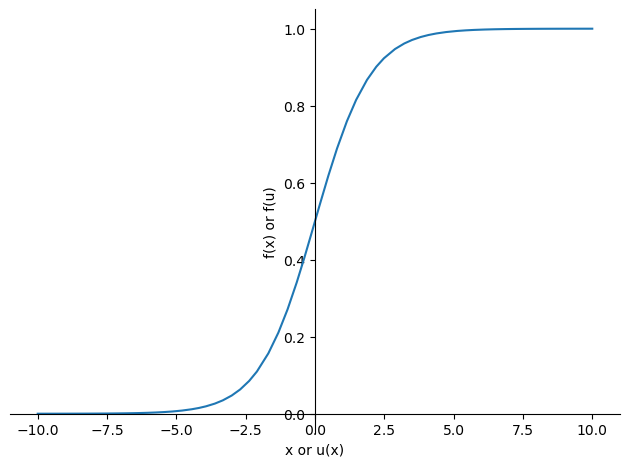
\includegraphics[width=0.5\textwidth]{Topic04fig01.png}
    \caption{Sigmoid function.}
    \label{t04fig01}
\end{figure}

The Sigmoid function has some interesting properties:
\begin{itemize}
    \item It is continuous and monotonically increasing over $\mathbb{R}$.
    \item $f(0) = \frac{1}{2}$.
    \item $f(x)$ ranges from 0 to 1:
    \[
    \lim_{x \to -\infty} f(x) = 0 \quad \text{and} \quad \lim_{x \to \infty} f(x) = 1.
    \]
\end{itemize}

Its first-order derivative has the following closed form:
\begin{equation}
\begin{split}
    \frac{\mathrm{d} f(x)}{\mathrm{d} x} & = \frac{\exp(-x)}{[1+\exp(-x)]^2}  \\
    & = f(x)[1 - f(x)]
\end{split}
\label{t04eq02}
\end{equation}

By letting $u(x)$ be a linear function, for example, $u(x) = w_0 + w_1 x$, we obtain the Logistic function parameterized by $\bm{w} = [w_0, w_1]^T$, which we denote as $f(x,\bm{w})$. That is,
\[
f(x, \bm{w}) = f[u(x)].
\]

Using the chain rule, the derivative of $f(x,\bm{w})$ with respect to a generic parameter $w$ is:
\begin{equation}
\begin{split}
    \frac{\partial f[u(x)]}{\partial w} & = \frac{\mathrm{d} f[u(x)]}{\mathrm{d} u(x)}\frac{\mathrm{d} u(x)}{\mathrm{d} w} \\
    & = f[u(x)]\Bigl[1 - f[u(x)]\Bigr] \frac{\mathrm{d} u(x)}{\mathrm{d} w}.
\end{split}
\end{equation}
For $\bm{w} = [w_0, w_1]^T$, we introduce the gradient notation:
\begin{equation}
\nabla_{\bm{w}} f(x,\bm{w}) = \begin{bmatrix}
      \frac{\partial f(u)}{\partial w_0} \\
      \frac{\partial f(u)}{\partial w_1} 
\end{bmatrix} = f(u)[1 - f(u)] \begin{bmatrix}
1\\
x
\end{bmatrix}.
\label{t04eq02b}
\end{equation}



\section{Learning from Data}
We start with a general dataset $\mathbf{D}$ defined as:
\[
\mathbf{D} = \{(x_k, c_k) \mid k = 1, 2, \ldots, N \}.
\]
For illustration, we introduce a toy dataset based on a water-quality experiment:
\[
\mathbf{D}_s = \{(x_k,c_k)\}_{k=1}^{3} = \{(3.0, 0), (5.0, 0), (7.0, 1)\}.
\]

As in the water-quality example, we expect to find a decision boundary—a function of $x$ or $u(x)$. Figure~\ref{t04fig04} illustrates decision functions expressed in different spaces: (a) in the original $x$ space; (b) as a function $u(x) = 0$ in a transformed space; and (c) in terms of the sigmoid function $f[u(x)]$.

\begin{figure}[ht]
    \centering
    \begin{subfigure}[b]{1\textwidth}
    \centering
    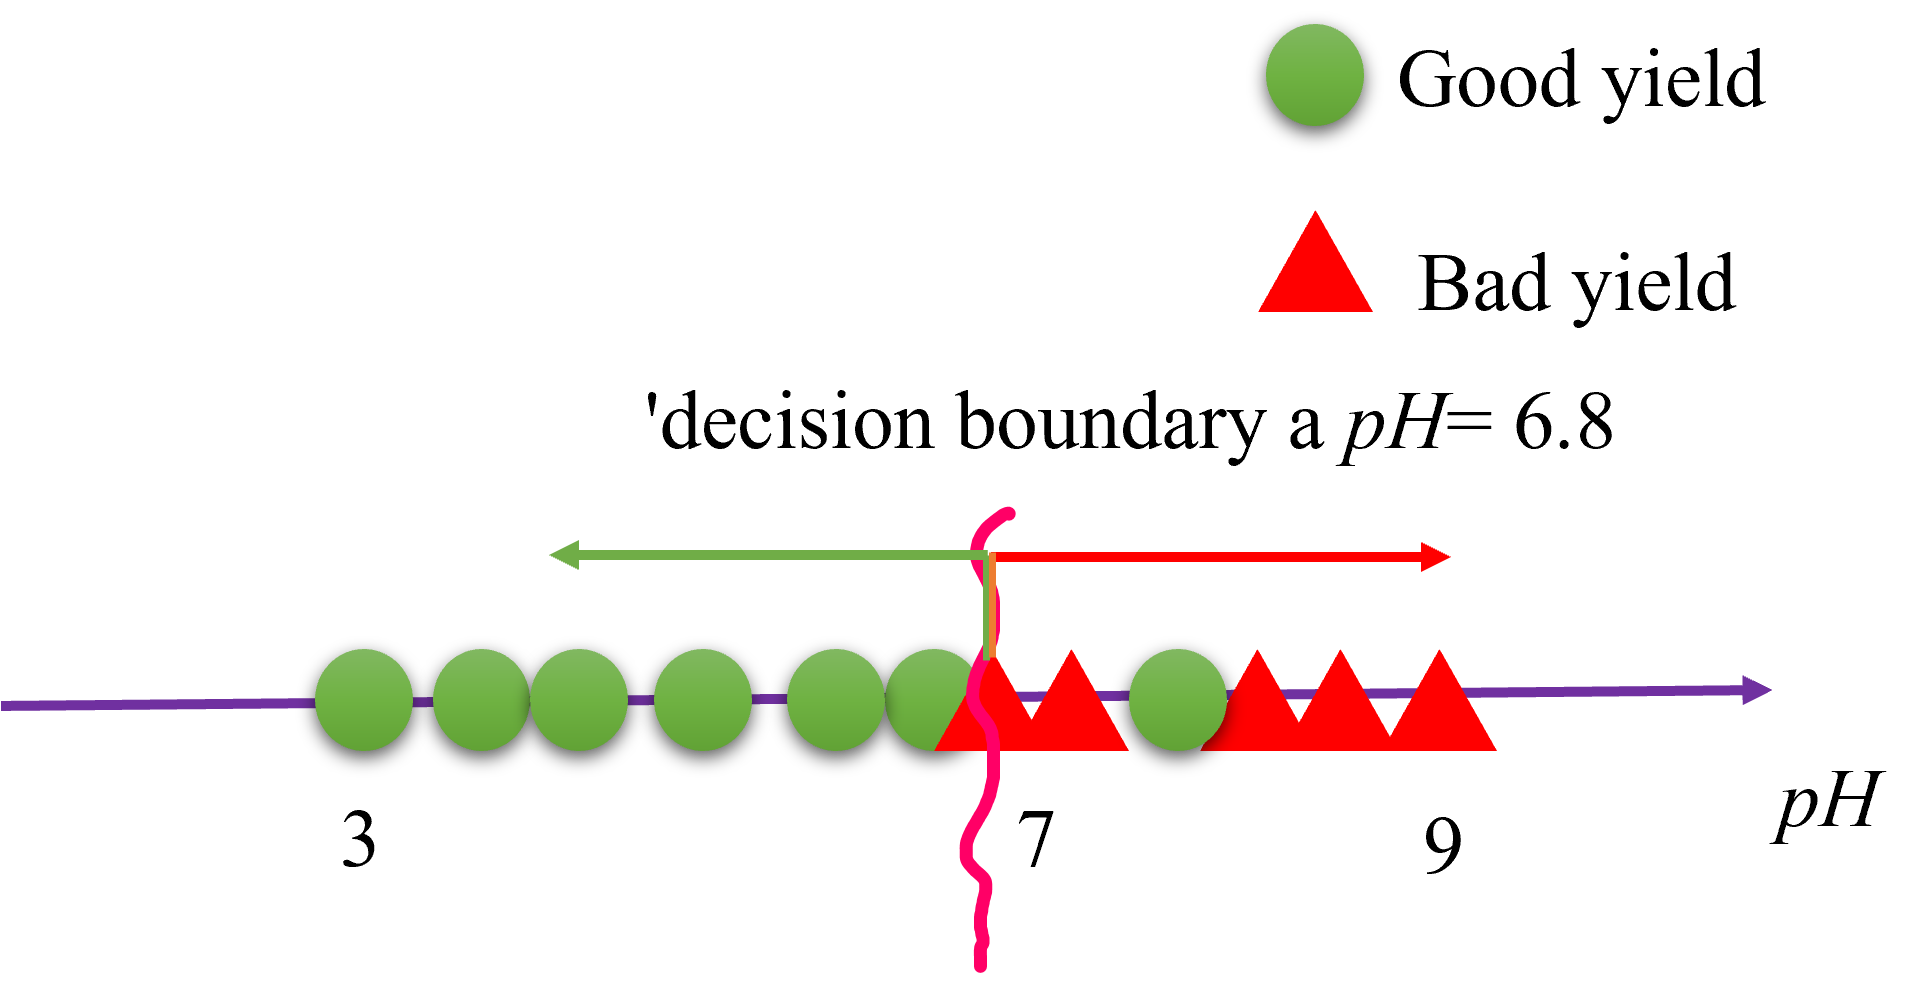
\includegraphics[width=0.5\textwidth]{Topic04fig04a.png}
    \caption{}
    \end{subfigure}
    \hfill
    \begin{subfigure}[b]{1\textwidth}
    \centering
    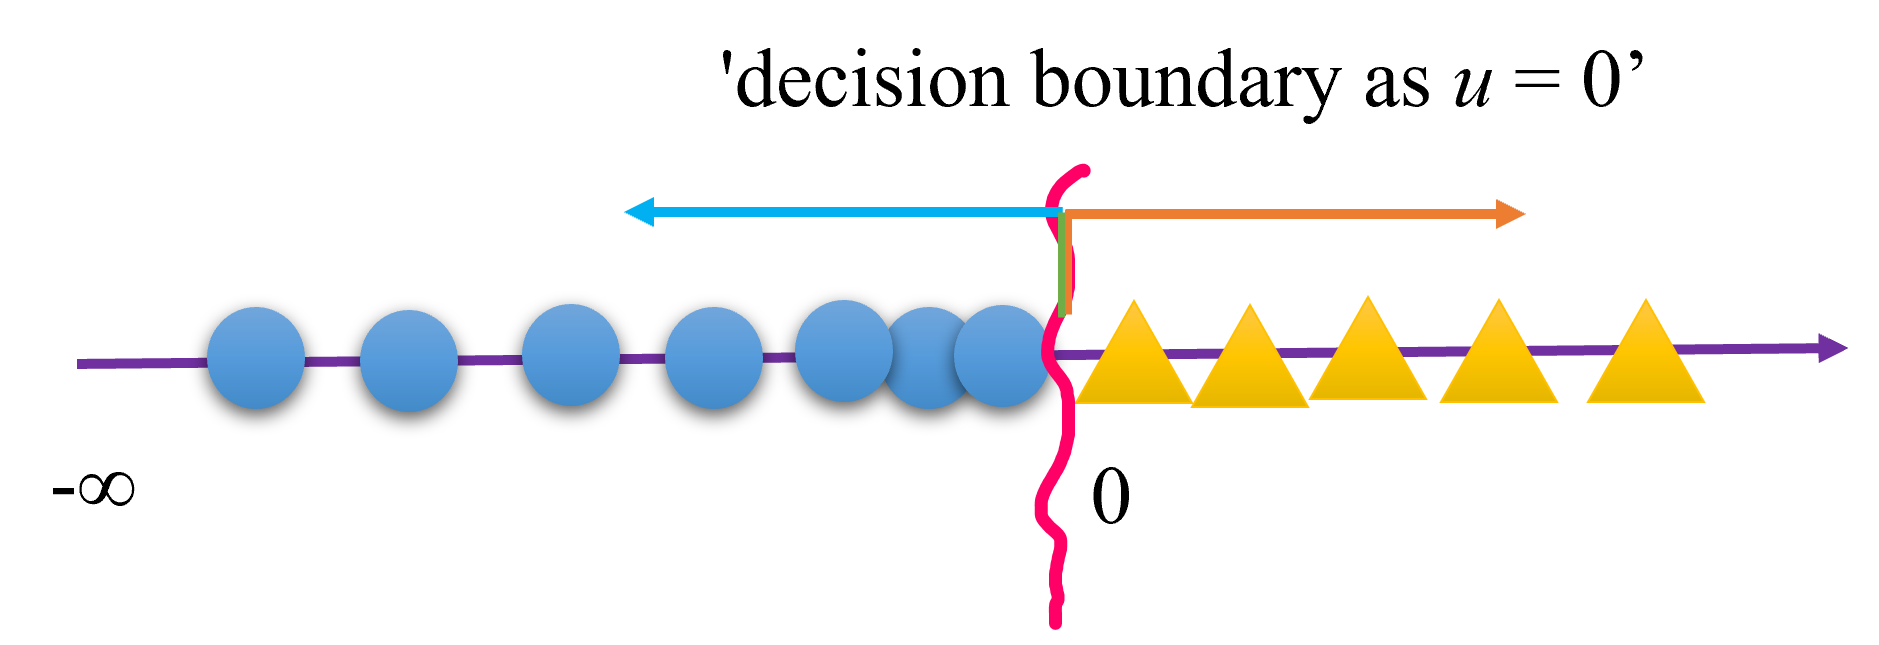
\includegraphics[width=0.5\textwidth]{Topic04fig04b.png}
    \caption{}
    \end{subfigure}
    \hfill
    \begin{subfigure}[b]{1\textwidth}
    \centering
    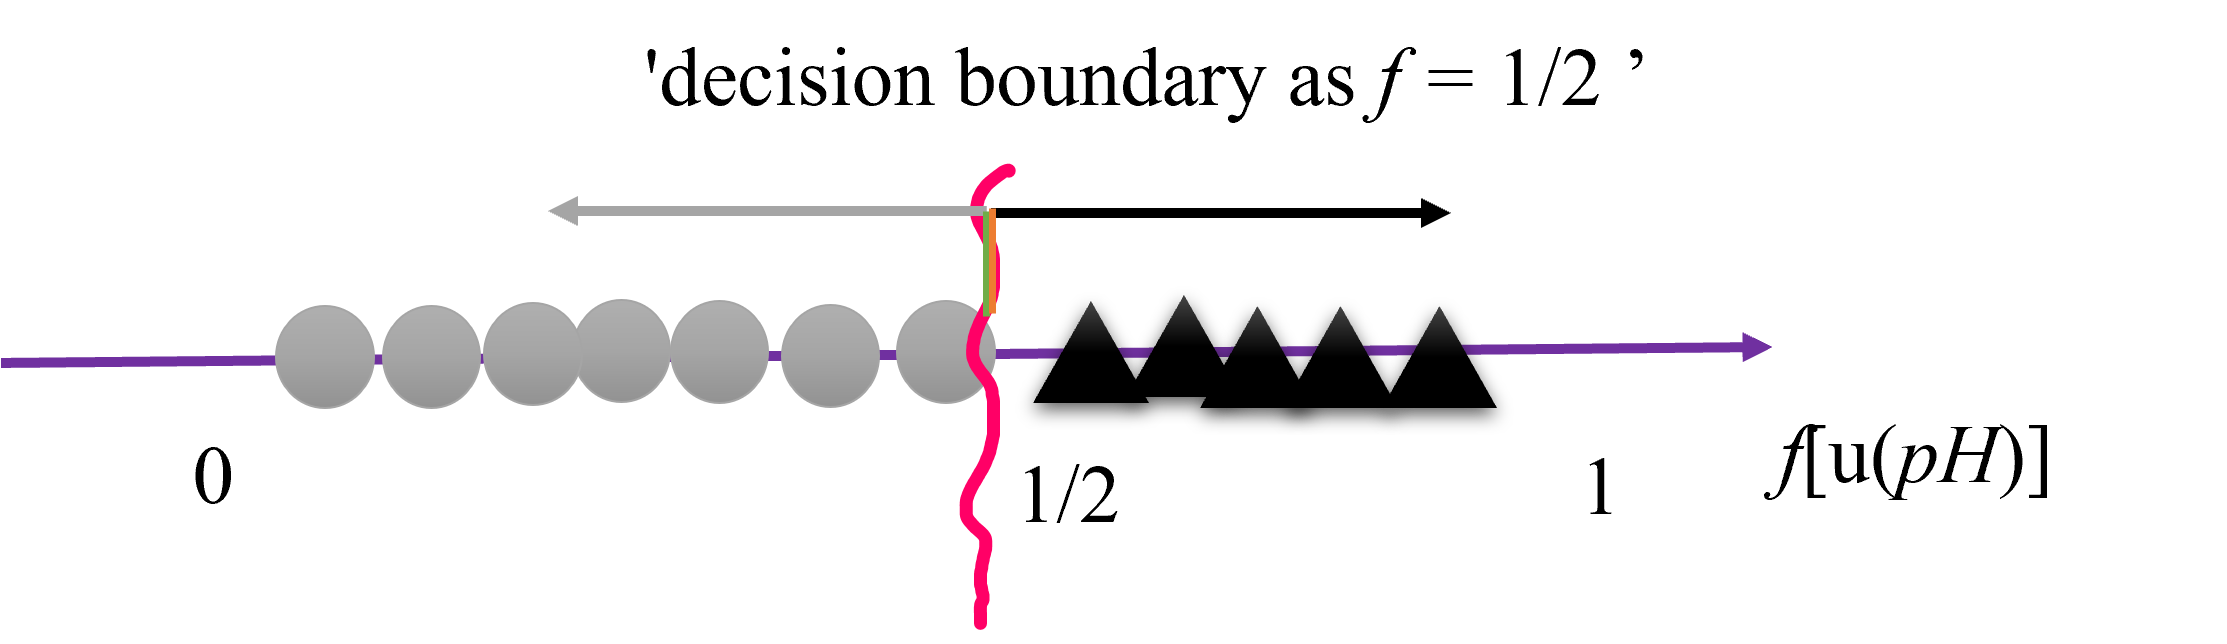
\includegraphics[width=0.5\textwidth]{Topic04fig04c.png}
    \caption{}
    \end{subfigure}
    \caption{Decision boundary functions at different levels: (a) in the original $x$ space; (b) as $u(x)=0$ in a transformed space; and (c) via the sigmoid function $f[u(x)]$, interpreted as a probability score.}
    \label{t04fig04}
\end{figure}

\subsection{Logistic Function as an ML Model}
The logistic function can be used as an ML model when the relation between an input $x$ and its label is simple and $x$ spans the full $\mathbb{R}$. Given any $x$, the function asymptotically approaches 0 as $x\to -\infty$ and 1 as $x\to \infty$, with a boundary value at $x=0$, where $f(x)=\frac{1}{2}$.

Thus, one can define a binary classifier:
\begin{equation}
    m(x|\bm{w}) = \begin{cases} 
      1 & \text{if } x \geq 0, \\
      0 & \text{if } x < 0,
    \end{cases}
    \label{t04eq03}
\end{equation}
or, equivalently, in terms of the logistic function:
\begin{equation}
    m(x|\bm{w}) = \begin{cases} 
      1 & \text{if } f(x) \geq \frac{1}{2}, \\
      0 & \text{if } f(x) < \frac{1}{2}.
    \end{cases}
    \label{t04eq04}
\end{equation}

In many practical cases the original feature $x$ may not span the entire real line (for example, a pH value ranges from 0 to 14). Therefore, a transformation is introduced:
\begin{equation}
    u(x) = w_0 + w_1 x,
    \label{t04eq05}
\end{equation}
which allows the logistic function to work effectively by shifting and scaling $x$. With this transformation, the classifier becomes:
\begin{equation}
    m(x|\bm{w}) = \begin{cases} 
      1 & \text{if } u(x) \geq 0, \\
      0 & \text{if } u(x) < 0,
    \end{cases}
    \label{t04eq06}
\end{equation}
or equivalently,
\begin{equation}
    m(x|\bm{w}) = \begin{cases} 
      1 & \text{if } f[u(x)] \geq \frac{1}{2}, \\
      0 & \text{if } f[u(x)] < \frac{1}{2}.
    \end{cases}
    \label{t04eq07}
\end{equation}
Here, $u(x)$ and $f[u(x)]$ represent decision functions in different spaces. In practice, $f[u(x)]$ is interpreted as the probability that $m=1$. For example, if $f=0.75$, the model estimates a 75\% probability for class 1.

\subsection{Decision Function Variants}
Besides using the linear transformation $u(x) = w_0 + w_1 x$ for a scalar $x$, more flexible decision functions may be required:
\begin{itemize}
    \item \textbf{Nonlinear Transformations:} A polynomial model (e.g., $u(x) = w_0 + w_1 x + \beta_2 x^2 + \cdots$) may be introduced when a linear decision function is insufficient.
    \item \textbf{Vector Inputs:} For multidimensional feature vectors $\bm{x} \in \mathbb{R}^d$, a common approach is to use an inner-product transformation:
    \begin{equation}
    u(\bm{x}) = \langle \bm{w}, \bm{x} \rangle + w_0 = \sum_{i=1}^{d} w_i x_i + w_0.
    \label{t04eq08}
    \end{equation}
    \item \textbf{Kernel Methods:} When linear transformations are inadequate in high-dimensional spaces, nonlinear transformations using kernel functions can be employed. This approach is fundamental to methods like support vector machines.
\end{itemize}

\subsection{Loss Function: A Design Process}
Assume we have the logistic regression model 
\[
f[u(x)] = f(u,\bm{w})
\]
with $\bm{w} = [w_0, w_1]$. For an input $x_k$, the model outputs a predicted probability $f_k=f(u_k)$, and a predicted label $c_{p,k}$ is assigned using a threshold of $\frac{1}{2}$. Comparing with the true label $c_k$, the simplest loss is the zero-one loss defined as $l_k = |c_{p,k} - c_k|$. 

However, for logistic regression a more refined loss is used. Consider a false-negative case ($f_k < \frac{1}{2}$, so $c_{p,k}=0$, with $c_k=1$); a smaller $f_k \ll \frac{1}{2}$ indicates a greater error. Hence, we define the logarithm loss:
\[
l_1(f_k) = -\ln(f_k).
\]
Similarly, for a false-positive case ($f_k \ge \frac{1}{2}$ with $c_{p,k}=1$ and $c_k=0$), we define:
\[
l_0(f_k) = -\ln(1-f_k).
\]
Combining both cases for a general $c_k \in \{0,1\}$, the loss function is:
\begin{equation}
    l(f_k) = -c_k \ln(f_k) - (1-c_k) \ln(1-f_k).
    \label{t04eq09}
\end{equation}
This loss is also known as the \emph{binary cross-entropy} (or \emph{negative log-likelihood}) loss. It arises naturally from maximum likelihood estimation: if we model the label as $c_k\sim\mathrm{Bernoulli}(f_k)$, then the conditional likelihood is
 \[
p(c_k \mid x_k, \bm{w}) = f_k^{c_k}(1-f_k)^{1-c_k},
 \]
and minimizing $-\ln p(c_k \mid x_k, \bm{w})$ yields Eq.~\eqref{t04eq09}.
Thus, the total loss over the dataset is:
\begin{equation}
    L = \sum_k l(f_k) = -\sum_k \left[ c_k \ln(f_k) + (1-c_k) \ln(1-f_k) \right].
    \label{t04eq11}
\end{equation}

Since $f_k=f(u_k)$ is a function of $w_0$ and $w_1$, the total loss $L$ is also a function of $\bm{w}$, i.e., $L = L(w_0, w_1)$.

Note that even for correct predictions there is a small loss, which encourages the model to improve its confidence.

\subsection{Optimization: The Final Step is Always Numerical}
Training the logistic regression model amounts to finding the parameter vector $\bm{w}^*$ that minimizes the total loss:
\begin{equation} 
\begin{split}
        \bm{w}^* & = \operatorname*{argmin}_{\bm{w}} L \\
        & = \operatorname*{argmin}_{\bm{w}} -\sum_k \left[ c_k \ln(f_k) + (1-c_k) \ln(1-f_k) \right].
\end{split}
\end{equation}

A common approach to this optimization problem is to use gradient-based methods. For a single data point, the gradient of the loss with respect to $\bm{w}$ is derived as follows:
\begin{equation}
\begin{split}
    \nabla_{\bm{w}} l(\bm{w}) & = \frac{\partial l}{\partial f(u)} \nabla_{\bm{w}} f(u) \\
    & = -\frac{c-f}{f(1-f)} \nabla_{\bm{w}} f(u) \\
    & = -\frac{c-f}{f(1-f)} \, f(u)[1-f(u)] \begin{bmatrix}
      \frac{\partial u}{\partial w_0} \\
      \frac{\partial u}{\partial w_1}
\end{bmatrix} \\
& = -(c-f)  \begin{bmatrix}
      1 \\
      x
\end{bmatrix},
\end{split}
\label{t04eq14}
\end{equation}
where $f=f(u)$ and we used the fact that $\frac{\partial u}{\partial w_0} = 1$ and $\frac{\partial u}{\partial w_1} = x$. 

For the entire dataset, the gradient becomes:
\begin{equation}
    \nabla_{\bm{w}} L = 
    \begin{bmatrix}
    \sum_k -(c_k - f_k) \\
    \sum_k -(c_k - f_k)x_k
    \end{bmatrix}.
    \label{t04eq15}
\end{equation}

Setting $\nabla_{\bm{w}} L = \bm{0}$ theoretically yields the optimal parameters. In practice, due to the nonlinearity of $f_k$, numerical iterative methods—such as gradient descent (or Newton's method when second-order information is available)—are used. The convexity of the loss function guarantees a unique global minimum.

\section{Toy Example} 
Consider a toy water-quality dataset:
\[
\mathcal{D} = \{(x_k, c_k) \mid k=1,2,3\} = \{(3.0, 0), (5.0, 0), (7.0, 1)\}.
\]
For this dataset, the logistic regression model is given by:
\[
f(x,\bm{w}) = \frac{1}{1+\exp(-w_0 - w_1 x)}.
\]
The total loss becomes:
\begin{equation*}
\begin{split}
    L & = -\sum_{k=1}^{3} \left[ c_k \ln(f_k) + (1-c_k) \ln(1-f_k) \right] \\
    & = -\left[ \ln(1-f_1) + \ln(1-f_2) + \ln(f_3) \right] \\
    & = -\ln \left[ (1-f_1)(1-f_2)f_3 \right],
\end{split}
\end{equation*}
where
\[
f_1 = \frac{1}{1+\exp(-w_0 - 3w_1)}, \quad
f_2 = \frac{1}{1+\exp(-w_0 - 5w_1)}, \quad
f_3 = \frac{1}{1+\exp(-w_0 - 7w_1)}.
\]

A surface plot of the total loss as a function of $w_0$ and $w_1$ is shown in Figure~\ref{t04fig07}.

\begin{figure}[ht]
    \centering
    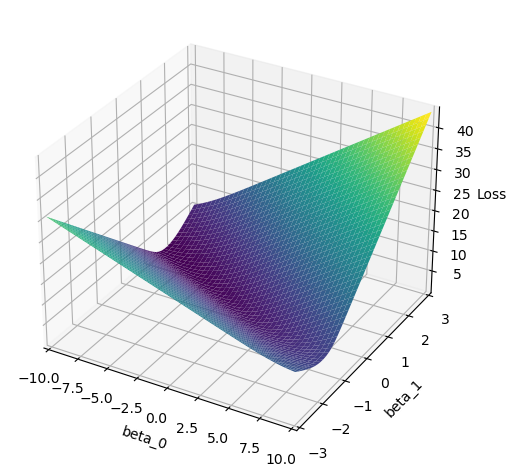
\includegraphics[width=0.5\textwidth]{Topic04fig07.png}
    \caption{The total loss function surface in terms of the model parameters $w_0$ and $w_1$.}
    \label{t04fig07}
\end{figure}

In practice, one would initialize the parameters and iteratively update $w_0$ and $w_1$ using a chosen step size following the gradient in Eq.~\ref{t04eq15}. The iterative process stops when further updates no longer reduce the loss. For this toy example, the parameter estimates are found to be:
\[
w_0 = -5.07184177, \quad w_1 = 0.81855117.
\]
Thus, the decision boundary defined by $u(x)=0$ becomes:
\[
0.81855117\,x - 5.07184177 = 0.
\]
Solving for $x$, we obtain:
\[
x^* \approx 6.1961,
\]
which aligns with the intuition from the training data: for $x > x^*$, the class label is predicted as 1; for $x < x^*$, it is 0.

\section{Conclusion}
In this lecture, we explored logistic regression as a fundamental discriminative model for binary classification. We began by reviewing its historical context and significance, noting its simplicity, interpretability, and computational efficiency. The derivation of the sigmoid and logistic functions laid the foundation for understanding how continuous probability outputs can be transformed into discrete class decisions. We then discussed the formulation of the decision function, including both linear and nonlinear transformations, and introduced the log-loss function as a principled way to quantify prediction errors. Finally, we demonstrated the complete process using a toy example, showing how parameter optimization via gradient-based methods yields a decision boundary that aligns with the training data. Overall, logistic regression not only serves as an essential baseline for more complex models but also provides valuable insights into the behavior and performance of discriminative classifiers in modern AI applications.

\end{document}
